\chapter{Localisation}
\section{Poincar\'e-Hopf theorem}
One of the primitive applications of the Mathai-Quillen formula is to prove the
Poincar\'e-Hopf theorem. 
Let $v\in\mathcal{X}(M)$ be a vector field on $M$.
At a zero $p\in M$ of  $v$, the Lie bracket of vector fields defines an endomorphism 
$\mathcal{L}_p(v) : T_pM \to T_pM$ by  $X\mapsto [X,v]$. In a coordinate system in
which  $p=0$ and  $v= v^i \partial_i$,  $\mathcal{L}_p(v)$ is given by 
 \[
	 \mathcal{L}_p(v)\partial_i = \sum_{j=1}^{n} [\partial_i, v^j(p)\partial^j] 
	 = \sum_{j=1}^{n} (\partial_i v_j(p)) \partial_j
\] 
A zero $p\in M$ is called \underline{non-degenerate} if  $\mathcal{L}_p(v)$ is
invertible. In this case, denote $\nu(p,v) = \sgn \det(\mathcal{L}_p(v)) 
\in \{\pm 1\}$. If all of the zeros of $v$ are non-degenerate, we call  $v$
non-degenerate. 

\begin{thm}[Poincare-Hopf] % Thm 1.56 BGV
	If $v$ is a non-degenerate vector field on an oriented compact manifold $M$ 
	of dimension $n$, then 
	\[
		 \int_M \chi(TM) = \sum_{\set{p|v(p)=0}} \nu(p,v)	
	\] 
\end{thm}
\begin{proof}
	(adapted from \cite[Theorem 1.56]{bgv})
	Choose a chart $\phi_p : U_p \to \mathbb{R}^n$ in a neighbourhood $U_p$ of
	each zero $p\in M$ of $v$, which gives coordinates on the tangent bundle 
	$\psi_p : TU_p \to \mathbb{R}^n$. The vector field $v$ defines a
	smooth map $\psi_p \circ v : U_p\to \mathbb{R}^n$ 
	with $v(p) = 0$ and invertible
	derivative $\mathcal{L}_p(v)$. 
	% TODO why is this the derivative?

	By the inverse function theorem, $v$ is a local diffeomorphism
	between open neighbourhoods $V_p \subset U_p$ and $B \subset \mathbb{R}^n$. 
	The orientation on $V_p$ induced by the oriented chart $\phi_p$ and by 
	the local diffeomorphism $\psi_p \circ v$ differ by the sign $\nu(p,v)$. 

	We may assume  $V_p$ are disjoint for each $p$.  Choose a Riemannian metric
	on $M$ which agrees with the metric on each $V_p$ induced by the diffeomorphism
	into  $\mathbb{R}^n$. Since $M$ is compact,  $\exists \epsilon > 0$ such
	that  $\norm{v} \geq \epsilon$ on the compact set  $M\setminus \bigcup_p V_p$,
	because if $\norm{v}$ can get arbitrarily close to 0, we would find a convergent
	subsequence in $M\setminus \bigcup_p V_p$ whose limit is a zero of $v$.  

	Let $U\in \Omega^n(TM)$ be the Mathai-Quillen Thom form of  $TM$ with respect to the
	Riemannian metric and associated Levi-Civita connection. 
	Let $f : \mathbb{R}_+ \to [0,1]$ be a smooth bump function such that $f(s)=1$
	if  $s < \epsilon^2 /4$ and $f(s)=0$ if  $s>\epsilon^2$. Then for all $t>0$
	\begin{equation} \label{eq:euler_zeros}
			\int_M \chi(TM) = \int_M v_t^* U 
		= \int_M (1-f(\norm{v}^2))v_t^*U  + \int_M f(\norm{v}^2)v_t^*U
	\end{equation}
	where $v_t := tv$. From equation (\ref{eq:MQ_exp}), we see that
	$v_t^* U$ is of the form
	\[
		v_t^*U = e^{-t^2\norm{v}^2 /2} \sum_{k=0}^{n} t^k \alpha_k
	\] 
	where $\alpha_k \in \Omega(M)$. Therefore, the first integral in equation
	(\ref{eq:euler_zeros}) is rapidly decreasing in $t$ since $\norm{v}^2 >
	\epsilon^2 /4$, and approaches zero as $t\to\infty$.

	On each $V_p$, the metric and connection are trivial since they are induced 
	by $v$. If we write $v= \sum_{i=1}^{n} x^i \partial_i$ in the coordinates of
	the chart $\psi_p$,
	\begin{align*}
		v_t^*U |_{V_p} 
		&= (2\pi)^{-n/2} e^{-t^2\norm{x}^2 /2} \int^B e^{-itdv} \\
		&= (2\pi)^{-n/2} \nu(p,v) e^{-t^2\norm{x}^2 /2} t^n dx^1 \wedge
		\ldots\wedge dx^n \tag{using Lemma \ref{lem:gaussian_integral}}
	\end{align*}
	The sign $\nu(p,v)$ comes from the Berezin integral using the orientation of
	the manifold, while $x^1,\ldots,x^n$ are coordinates of the vector field. 
	Therefore, 
	\begin{align*}
		\lim_{t \to \infty} \int_{V_p} f(\norm{v}^2)v_t^*U 
		&= (2\pi)^{-n/2} \nu(p,v) 
		\lim_{t \to \infty} \int_{\mathbb{R}^n}
		f(\norm{x}^2) e^{-t^2\norm{x}^2 /2} t^n dx^1 \wedge \ldots\wedge dx^n\\
		&= (2\pi)^{-n/2} \nu(p,v) 
		\lim_{t \to \infty} \int_{\mathbb{R}^n} 
		f(\norm[*]{t^{-1}y}^2) e^{-\norm{y}^2 /2} dy^1 \wedge \ldots\wedge dy^n\\
		&= \nu(p,v) 
	\end{align*}
	where we have made the change of variables $x=t^{-1}y$. Summing over each of
	the neighbourhoods $V_p$ of zeros, we get the result.
\end{proof}

There is a generalisation of this result, where we assume that the zeros
of $v$ are isolated instead of non-degenerate.\cite[Theorem 1.58]{bgv} 
It is desirable to generalise this further to relate the Euler number of
arbitrary vector bundles to zeros of a section, but the Poincar\'e-Hopf theorem
relies on the Lie bracket of vector fields to define the orientation of each
zero. In order to describe such a generalisation we first need to introduce some
intersection theory.

\section{Poincar\'e dual as a Thom class}
% p51 Bott Tu
Let $M$ be an oriented manifold and $i: S \xhookrightarrow{} M$ be a compact,
oriented submanifold with $\dim S = k, \dim M = n$. 
Poincar\'e duality (Theorem \ref{thm:poincare_duality}) can be used to associate 
$S$ to a unique cohomology class $[\eta_S]\in H^{n-k}_c(M)$ called its
\underline{Poincare dual} as follows. Define the linear functional
\[
H^k(M) \to \mathbb{R}, \qquad 
\omega \mapsto \int_S i^*\omega
\] 
Here $\int_S i^*\omega$ is defined because $S$ is compact. 
It follows by Poincare duality that integration over $S$ corresponds to a
unique cohomology class $[\eta_S]\in H^{n-k}_c(M)$, with the property that 
for any $\omega\in H^k(M)$
\begin{equation} \label{eq:poincare_dual_property}
	\int_S i^*\omega = \int_M \omega \wedge \eta_S
\end{equation}
\begin{remark} % TODO and closed (as a subspace) needed?
	The same argument can be applied to define the Poincar\'e dual of an
	oriented submanifold $S \subset M$ that is not
	necessarily compact. This is associated to a linear functional 
	$H^k_c(M) \to \mathbb{R}$ by integrating over $S$. This is well defined
	because for any	compact $K\subset M$, $K\cap S$ is compact in $S$.
	This corresponds to a unique cohomology class $[\eta_S] \in H^{n-k}(M)$,
	satisfying equation (\ref{eq:poincare_dual_property}) for $\omega \in
	H^k_c(M)$.
\end{remark}
Notice that the Poincar\'e dual has a remarkably similar property to the 
Thom class (c.f. equation (\ref{eq:thom_form_property})). 
To relate the two ideas, this requires constructing a vector bundle over the
submanifold $S$, which leads to the concept of a tubular neighbourhood.
\begin{defn}
	The \underline{normal bundle} of $S$ in  $M$ is the quotient vector bundle
	$N_S\to S$ defined by the exact sequence 
	\[
	\begin{tikzcd}[column sep = 1.6em]
		0 \arrow[r] & TS \arrow[r] & TM|_S \arrow[r] 
						& N_S \arrow[r] & 0
	\end{tikzcd}
	\]
	Let $S \subset M$ be a submanifold. 
	A \underline{tubular neighbourhood} of  $S$ in  $M$ is an open
	neighbourhood of  $S$ in  $M$ diffeomorphic to the normal bundle of $S$ in
	 $M$, such that  $S$ is diffeomorphic to the zero section.
\end{defn}
For a Riemannian manifold, one can identify $N_S$ with the orthogonal
complement. If we further assume $S$ and $M$ are oriented, then there is an
induced orientation on the normal bundle via 
\begin{equation} \label{eq:normal_orientation}
	\operatorname{or}(TM|_S) = \operatorname{or}(TS)\wedge \operatorname{or}(N_S)
\end{equation}
where $\operatorname{or}(N_S)$ denotes the orientation form on the vector bundle. 

% https://luis.impa.br/aulas/anvar/Spivak_Vol1_3ed.pdf Spival p346
% https://www.math.tecnico.ulisboa.pt/~acannas/Books/lsg.pdf p37
% \cite[Theorem 6.5]{anacannas}
% http://alpha.math.uga.edu/~usher/8210-notes2.pdf Thm 2.11
\begin{thm}[Tubular neighbourhood theorem {\cite[Thm 5.25]{riemannian_manifolds}}] 
	Every submanifold $S$ of a Riemannian manifold $M$ has a 
	tubular neighbourhood  $T\subset M$. If $S$ is compact, the tubular
	neighbourhood can be chosen to have constant radius.
\end{thm}
\begin{comment}
\begin{proof}[Proof (sketch).]
	Let $V\subset TM$ be the domain of the exponential map, and 
	The idea is that for each $x\in S$, the exponential map is a diffeomorphism
	on a neighbourhood of $x$
	\[
		V_\delta(x) = \{(x',v')\in N_S \mid d_g(x,x')<\delta, \abs{v'}_g<\delta\}
	\] 
	for some $\delta$. It can be shown that 
	 \[
		 \Delta(x) = \sup \{\delta \leq 1 \mid \exp \text{ is a diffeomorphism
		 from} V_\delta \text{ to its image}\}
	\] 
	is a continuous function $\Delta : S \to \mathbb{R}$. Then 
	\[
		U = \{(x,v)\in N_S \mid \abs{v}_g < \frac{1}{2}\Delta(x)\}
	\] 
 	is a neighbourhood of $N_S$ containing the zero section $S$. It can be shown
	that  $\exp$ is injective on  $U$. Therefore  $\exp$ is a diffeomorphism
	from  $U$ to its image  $T$, which shows that  $T$ is a tubular
	neighbourhood.
\end{proof}
\end{comment}
\begin{figure}[htb]
	\hfill
	\begin{minipage}[c]{0.56\textwidth}
		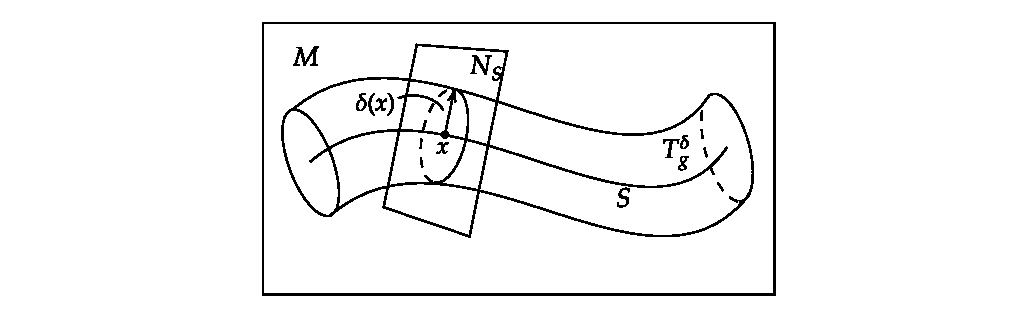
\includegraphics[trim={4cm 3mm 4cm 3.7mm},clip,width=\textwidth]{figs/tubular_neighbourhood.pdf}
	\end{minipage} 
	\begin{minipage}[c]{0.3\textwidth}
        \caption{A tubular neighbourhood}
        \label{fig:tubular_neighbourhood}
	\end{minipage} 
\end{figure}
The proof of the theorem shows that the tubular neighbourhood is the
diffeomorphic image under the exponential map of a subset of the form
\begin{equation} \label{eq:tubular_radius}
	V^\delta_g = \set[*]{(x,v)\in N_S \mid \abs{v}_g < \delta(x)}
	\;\mapsto\; 
	T^\delta_g = \set{x \in M \mid \operatorname{dist}_g(x,S) < \delta(x)}
\end{equation}
for some positive smooth function $\delta : S \to \mathbb{R}$, called the
radius, which can be chosen as small as desired. Note that $V^\delta_g$ is 
diffeomorphic to  $N_S$. In this construction, the fiber over $x\in S$ is
\begin{equation} \label{eq:tubular_fiber}
		T^\delta_g(x) = \{z \in M \mid \operatorname{dist}_g(z,S) 
		= d_g(z,x) < \delta(x)\}
\end{equation}

We can now explain the relation between the Poincar\'e dual and Thom class.
Let $S$ be an oriented submanifold of an oriented manifold $M$. 
% which is closed as a subspace. % Not using closed homology, see BottTu p51 
If $j:T \hookrightarrow M$ is the inclusion of a tubular 
neighborhood of $S$, we have a Thom class $U \in H^{n-k}_{cv}(T)$ by identifying 
$T$ with the normal bundle of $S$. 
We can define a map $j_*:H_{cv}^{*}(T) \to H^*(M)$ which extends by zero,
because forms that are compactly supported along the fiber go to zero near 
the boundary of $T$. 
% The following theorem illuminates the relation between the Poincar\'e dual 
% and Thom class: % repetitive

\begin{thm}[Poincar\'e dual as a Thom class] \label{thm:poincare_thom} % p67 Bott Tu
	The Poincar\'e dual $\eta_S$ of $S$ is equal to the Thom class 
	$U\in H^{n-k}_{cv}(T)$ of the
	tubular neighbourhood of $S$. That is, 
	\[
		\int_M \omega\wedge j_*U = \int_S i^*\omega \qquad
		\text{for all } \omega\in H^k(M)
	\] 
	where $U$ is defined by identifying 
	$T$ with the normal bundle.
\end{thm}
\begin{proof}
	Let $\omega \in H^k(M)$. Consider $\omega$ as a form on  $T$, since
	we are not concerned with its values outside this region, so we may view
	the inclusion $i : S \to T$ as the zero section. Note that $\pi : T \to S$
	induces a deformation retraction of $T$ onto $S$, so $\pi$ and  $i$
	are inverse isomorphisms in cohomology. This means $\omega$ differs from
	$\pi^*i^*\omega$ by an exact form:  $\omega = \pi^*i^*\omega + d\tau$.
	\begin{align*}
		\int_M \omega\wedge j_*U 
		= \int_T \omega \wedge U 
		&= \int_T (\pi^*i^*\omega + d\tau) \wedge U \\
		&= \int_T (\pi^*i^*\omega) \wedge U \tag{by Stokes' theorem}\\
		&= \int_S i^*\omega  \wedge \pi_*U 
		\tag{by Proposition \ref{prop:projection_formula}}\\
		&= \int_S i^*\omega \tag{since $\pi_*U = 1$} 
	\end{align*}
\end{proof}
\vspace{-1.5ex}
In particular, this means that the Poincar\'e dual of the image of the zero 
section $M_0\subset E$ of a vector bundle $E\to M$ is the equal to the Thom 
class of  $E$. This is because the exact sequence 
\[
	\begin{tikzcd}[column sep = 1.6em]
		0 \arrow[r] & TM_0 \arrow[r] & TE|_{M_0} \arrow[r] 
						& E \arrow[r] & 0
	\end{tikzcd}
	\]
shows that the normal bundle of the zero section is  $E$ itself.  

\begin{remark}[Localisation principle]
	Another observation is that the support of the Poincar\'e dual of $S$ can be
	shrunk into any arbitrarily small tubular neighbourhood of $S$, 
	by simply pulling back the Thom class of the
	normal bundle into the tubular neighbourhood.
\end{remark}

To find the Poincar\'e dual of the zero set of an arbitrary section, or more
generally the inverse image of a submanifold, we first need a result 
in intersection theory.
It will be useful at this stage to review transversality in Appendix
\ref{appendix4} before continuing. 

\section{Poincar\'e dual of submanifolds}
\begin{defn} % def 2.5 nicolescu
	Let $S$ and  $L$ be oriented submanifolds of the
	oriented manifold  $M$ such that  $\dim S + \dim L = \dim M$. Suppose 
	 $S$ and  $L$ intersect transversely. Then for each  $p\in L\cap S$, define
	 $\epsilon(S,L,p) \in \{\pm 1\}$ via
	 \[
		 \operatorname{or}(T_pS) \wedge \operatorname{or}(T_pL)
		 = \epsilon(S,L,p) \operatorname{or}(T_p M)
	 \] 
	 If $S\cap L$ is finite, we can define the
	 \underline{intersection number} of  $L$ and  $S$ to be the integer
	  \[
		  [S]\cdot [L] = \sum_{p\in S\cap L} \epsilon(S,L,p)
	 \] 
\end{defn}
\begin{remark}
	One way to guarantee that $S\cap L$ is finite is when $S\cap L$ is compact. 
	Theorem \ref{thm:inverse_submanifold} applied to
the inclusion $i: S \to M$ and  $L$ tells us that  $S\cap L$ is a zero
dimensional submanifold. If $S\cap L$ is not finite, there is a sequence  
$(x_n)_{n\in \mathbb{N}} \subset S\cap L$ such that $x_n \to x \in S\cap L$. So 
there is no neighbourhood of $x$ in $M$ whose restriction to $S\cap L$ is a
point, contradicting that $S\cap L$ is a zero dimensional submanifold. 
\end{remark}

\begin{thm} \label{thm:intersection_poincare} % nicolescu theorem 2.6 p7
	Suppose $S$ and  $L$ are oriented submanifolds of the 
	oriented manifold  $M$, and $S$ or $L$ is compact.
	Assume  $S \pitchfork L$ and  $\dim L + \dim S = \dim M$.
	Then 
	\[ 
		[S] \cdot [L] = \int_M \eta_S \wedge \eta_L = \int_L \eta_S
	\] 
\end{thm}
\begin{proof}
	Set $s=\dim S$, $l=\dim L$ and $n=s+l$. For any $p\in S\cap L$, there are
	submersions $f : U_p \to \mathbb{R}^l$ and $g:U_p\to \mathbb{R}^s$ from a
	neighbourhood of $p$ such that  $f^{-1}(0) = S \cap U_p$ and $g^{-1}(0) =
	L\cap U$. Then the joint function $\psi=(g,f) : U_p \to \mathbb{R}^n$ satisfies 
	\[
		S\cap U_p = \{x_{s+1}=\cdots=x_{s+l}=0\}, \quad
		L\cap U_p = \{x_{1}=\cdots=x_{s}=0\}, 
	\] 
	Since $\dim M = l + s$ and $S\pitchfork L$, the tangent space is a direct sum 
	$T_pM = T_pS \oplus T_pL$. Since $f$ and  $g$ are also submersions,
	it follows that $D\psi|_p : T_p S \oplus T_p L \to \mathbb{R}^{s+l}$ is 
	bijective. Hence, by the
	inverse function theorem, we can assume $\psi$ is a diffeomorphism to its
	image. 

	\begin{comment}
	By permuting the components if necessary, assume that orientation of $S\cap
	U_p$ is described in coordinates as $dx_1\wedge\cdots\wedge dx_s$, while the 
	orientation of $L\cap S$ is $dx_{s+1}\wedge \cdots\wedge dx_{s+l}$.
	\end{comment}
 	\begin{figure}[htb]
		\hfill
 		\begin{minipage}[c]{0.6\textwidth}
			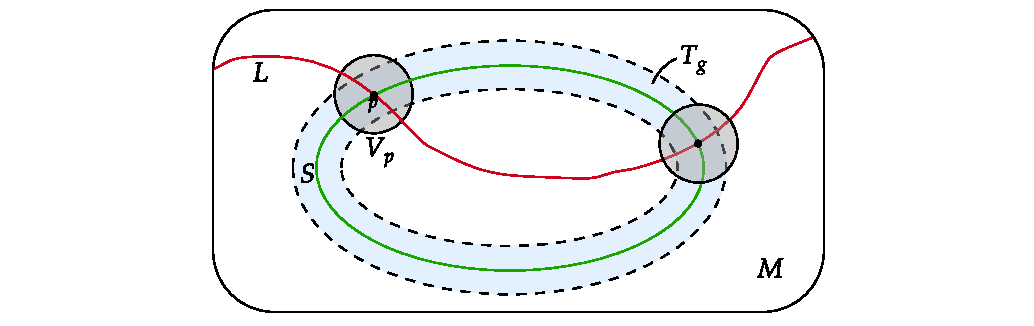
\includegraphics[trim={35mm 0 35mm 0},clip,width=\textwidth]{figs/tubular_intersection.pdf}
 		\end{minipage} 
 		\begin{minipage}[c]{0.38\textwidth}
 	        \caption{The fibers of the tubular neighbourhood of $S$ at points of
			transverse intersection coincides with  $L$}
 	        \label{fig:tubular_intersection}
 		\end{minipage} 
 	\end{figure}	
	Our key idea is that we can choose neighbourhoods $V_p \subset U_p$
	and a Riemannian metric $g$ on  $M$ such that on $V_p$ the metric is the
	Euclidean norm $(dx_1)^2 + \ldots+(dx_n)^2$. This means that we can choose a
	tubular neighbourhood $T_g \subset M$ of $S$  such that the fibers coincide
	with the submanifold $L$, i.e. (see Figure \ref{fig:tubular_intersection})
	\[
	T_g(p) = (L \cap V_p) \cap T_g
	\] 
	where we must choose $T_g$ small enough so that the fiber of $p$ is 
	contained in $V_p$. Note we can assume $V_p$ are disjoint, so that $L\cap
	T_g = \bigcup_{p\in S\cap L} T_g(p)$. Let $\eta_S \in \Omega^l(M)$ be a
	representative of the Poincar\'e dual of $S$ with support on  $T_g$. 
	
	The fiber $T_g(p)$ is equipped with the co-orientation of  $S$ in $M$
	(equation (\ref{eq:normal_orientation})). 
	Denote $L_p := T_g(p)$ to be the same fiber but equipped with the
	orientation induced by  $L$. Then we have the relation 
	\[
		\operatorname{or}(L_p) = \epsilon(S,L,p) \operatorname{or}(T_g(p))
	\] 
	Now observe that 
	\[
	\int_M \eta_S \wedge \eta_L 
	= \int_L \eta_S
	= \sum_{p\in S\cap L} \int_{L_p} \eta_S
	= \sum_{p\in S\cap L} \epsilon(S,L,p)\int_{T_g(p)} \eta_S
	= \sum_{p\in S\cap L} \epsilon(S,L,p)
	\] 
	where $\int_{T_g(p)}\eta_S = 1$ by Theorem \ref{thm:poincare_thom}.
\end{proof}

\begin{comment} % Poincare dual for smooth cycles
We can generalise the notion of Poincar\'e dual of submanifolds to smooth
cycles.  The pair  $(N,f)$ determines a linear
functional 
\[
H^n(M) \to \mathbb{R}, \qquad \omega \mapsto \int_N f^*\omega
\] 
The integral is well defined because $N$ is compact. We call this linear
functional a smooth cycle, and denote it $f_*[N]$. As before, it follows by
Poincar\'e duality that integration over $N$ corresponds to a unique
$[\eta_{f_*[N]}] \in H^{m-n}(M)$ such that 
\[
	\int_N f^*\omega = \int_M \omega \wedge \eta_{f_*[N]} \quad\; 
	\fall \omega \in H^n(M)
\] 
\end{comment}

We can generalise Theorem \ref{thm:poincare_thom} 
by finding the Poincar\'e dual of the zero set of an arbitrary section, or more
generally the inverse image of a submanifold.

Suppose $M$ and $N$ are oriented manifolds of dimensions $m$
and $n$, $f:N\to M$ is a smooth map, and
$S \subset M$ is a submanifold of dimension $k$ that is transverse to $f$. 
By Theorem \ref{thm:inverse_submanifold}, $f^{-1}S\subset N$ is a submanifold 
of dimension $n-m+k$, assuming of course that $n+k \geq m$. 
The following lemma gives an orientation on the normal
bundle $N_{f^{-1}(S)}$, which in turn gives a natural orientation on $f^{-1}(S)$
via equation (\ref{eq:normal_orientation}). 

\begin{lem} \label{lem:normal_isomorphism}
	There is a bundle isomorphism $Df : N_{f^{-1}(S)} \to f^*N_{S}$.
\end{lem}
\begin{proof}
	First observe that $f \pitchfork S$ if and only if  $Df|_x : T_x N \to
	T_{f(x)}M$ maps surjectively to the quotient vector space $T_{f(x)}M /T_{f(x)} S =
	(N_S)_{f(x)}$ for all $x\in f^{-1}(S)$. Note that $Df|_x$ maps
	$T_xf^{-1}(S)$ into $T_{f(x)}S$ (this is true in general), and hence
	the kernel of the map $Df|_x : T_x N \to (N_S)_{f(x)}$ is $T_xf^{-1}(S)$. 
	The kernel cannot be any larger due to dimension constraints from
	surjectivity. Therefore, by the first isomorphism theorem 
	$Df|_x : (N_{f^{-1}(S)})_x \to (N_S)_{f(x)}$ is a linear
	isomorphism. Consequently, 
	$Df : N_{f^{-1}(S)} \to f^*N_{S}$ is a bundle isomorphism. 
\end{proof}


\begin{thm} % nicolescu thm 3.4 % Bott Tu pg 69 
	Let $f : N \to M$ and  $S \subset M$ as above such that $f^{-1}(S)$ is
	compact. Then $f^*\eta_S = \eta_{f^{-1}(S)}$,  i.e. 
	\[
	\int_{N} \omega \wedge f^*\eta_S =\int_{f^{-1}(S)} i^*\omega  
	\qquad
	\text{for all }\omega\in H^{n-m+k}(N)
	\]
	where $i: f^{-1}(S) \to N$ is the inclusion map.
\end{thm}
\begin{proof} 
	Fix Riemannian metrics $g$ on $N$ and $h$ on $M$.
	Let $T^\epsilon_g \subset N$ and $T^\delta_h \subset M$ be tubular
	neighbourhoods of  $f^{-1}(S)$ in $N$ and  $S$ in $M$, of the form in
	equation (\ref{eq:tubular_radius}). Since $f^{-1}(S)$ is compact, assume  
	$\epsilon$ is constant. Denote by $T^\epsilon_g(x)$ the fiber over 
	$x\in f^{-1}(S)$,
	defined in equation (\ref{eq:tubular_fiber}). 
	We claim that there exists $\epsilon > 0$ such that the restriction of  $f$
	to  $T^\epsilon_g(x)$ is diffeomorphism to its image for all  
	$x\in f^{-1}(S)$. % lemma 3.5
	\begin{subproof}
		By Lemma \ref{lem:normal_isomorphism}, 
		$Df|_x : (N_{f^{-1}(S)})_x \to (N_S)_{f(x)}$ is an isomorphism.
		By identifying the fiber $(N_{f^{-1}(S)})_x$ as the tangent space to 
		the fiber of the tubular neighbourhood, we can write  
		$Df|_x : T_xT_g^\epsilon(x) \to T_{f(x)}T_h^\delta(f(x))$. 
		This can be interpreted as the differential of the restriction to
		$T^\epsilon_g(x)$. 
		So by the inverse function theorem, for each $x\in f^{-1}(S)$,
		there exists a neighbourhood $U_x \subset N$ of $x$ and  $\epsilon(x)>0$
		such that the restriction to  $T^{\epsilon(x)}_g(x)$ is a diffeomorphism
		to its image. Since $f^{-1}(S)$ is compact, there is a finite subcover 
		$U_{x_1},\ldots,U_{x_r}$ and define 
		$
			\epsilon = \min\{\epsilon(x_1),\ldots,\epsilon(x_r)\}
		$. 
	\end{subproof}
	\begin{figure}[htb]
		\centering
		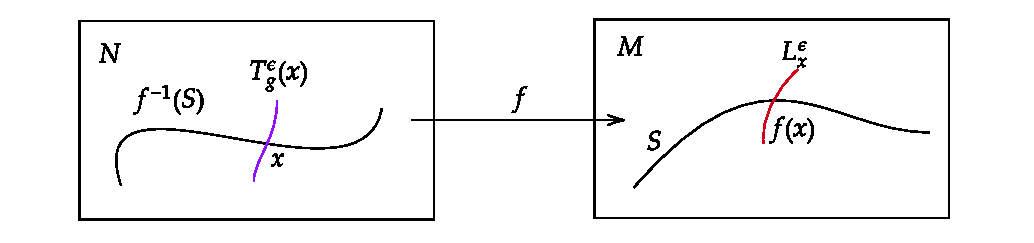
\includegraphics[width=\textwidth]{figs/normal_fiber_map.pdf}
		\caption{The diffeomorphism $f:T^\epsilon_g(x) \to L_x^\epsilon$ mapping
		the normal fiber}
		\label{fig:normal_fiber_map}
	\end{figure}
	For such an $\epsilon$,  denote the image of the embedding  $L_x^\epsilon :=
	f(T^\epsilon_g(x))$. 

	\begin{comment} % TODO needed?
	Next, we claim that there exists 
	$\rho > 0$ such that for any  $x\in f^{-1}(S)$ the intersection 
	$L_x^\epsilon \cap T_h^\rho$ is closed in $T^\rho_h$.
	Note that $T^\rho_h$ is not necessarily a tubular neighbourhood of $S$.
	\begin{subproof}
		Denote the boundary of the tubular neighbourhood $\Sigma_\epsilon = \{z\in
		N \mid \operatorname{dist}_g(z,f^{-1}(S)) = \epsilon\}$. 
		Then $f(\Sigma_\epsilon)$ is a compact image of a compact set, and is
		disjoint from $S$.  Thus, 
		$\operatorname{dist}_h(f(\Sigma_\epsilon),S) > 0$.

		We will show $\rho = \frac{1}{2}\operatorname{dist}_h(f(\Sigma_\epsilon),S)$
		is the desired value. Suppose $(y_n)_{n\in \mathbb{N}} \subset 
		L_x^\epsilon \cap T_h^\rho$ is a sequence that converges to $y\in T^\rho_h$. 
		We need to show $y\in L_x^\epsilon$. We can choose points 
		 $p_n \in T^\epsilon_g(x)$ such that $f(p_n) = x_n$. Since  $f^{-1}(S)$ is
		 compact, there is a subsequence which converges to a point $p$ such
		 that $d_g(p,x) \leq \epsilon$. Since $y$ is the unique limit, we have 
		 $f(p) = y$. And since $\operatorname{dist}_h(y_n,S) < \rho$,   
		 \[
			 \operatorname{dist}_h(y,S) \leq \rho < \dist_h(f(\Sigma_\epsilon),S)
		 \] 
		Then $f(p) \notin f(\Sigma_\epsilon)$ implies $p\notin \Sigma_\epsilon$,
		i.e. $d_g(p,x) < \epsilon$ is a strict inequality. Thus  $p\in
		T^\epsilon_g(x)$ so $y\in L_x^\epsilon$.
	\end{subproof}
	Replace $\delta$ with a smooth function bounded above by $\min(\delta(x),\rho)$ 
	so that the above holds, and $T_h^\delta$ is a tubular neighbourhood.
	\end{comment}

	Choose a form $\eta_S$ representing the Poincar\'e dual with support in
	$T^\delta_h$. The integral of $f^*\eta_S$ along the fiber  $T^\epsilon_g(x)$
	is 
	 \[
	\int_{T^\epsilon_g(x)} f^*\eta_S 
	= \int_{L_x^\epsilon} \eta_S = [S] \cdot [L_x^\epsilon] = 1
	\] 
	The first equality applies via the diffeomorphism
	$f:T^\epsilon_g(x) \to L_x^\delta$. 
	The second equality follows from Theorem \ref{thm:intersection_poincare},
	since $L_x^\epsilon$ is compact.
	
	Therefore, $f^*\eta_S$ is the pullback of Thom class of the normal bundle over
	$f^{-1}(S)$, so it is equal to the Poincar\'e dual of $f^{-1}(S)$ by Theorem 
	\ref{thm:poincare_thom}.
\end{proof}
\begin{comment} % old proof using Bott Tu
\begin{proof}
	Bott Tu version:
	Also $f^{-1}T \subset N$ is a neighbourhood of 
	dimension $n$ (why?). 
	We can choose $T$ to be a sufficiently small tubular
	neighbourhood of  $S$ such that  
	$f^{-1}T$ is contained within a tubular
	neighbourhood of $f^{-1}S$ in $N$, and hence diffeomorphic to 



	The following diagram commutes (why?)
	% https://q.uiver.app/?q=WzAsNixbMCwwLCJIXiooUykiXSxbMSwwLCJIXnsqK2t9KFQpIl0sWzIsMCwiSF4qKE0pIl0sWzIsMSwiSF4qKE0nKSJdLFsxLDEsIkheeyora30oZl57LTF9VCkiXSxbMCwxLCJIXiooZl57LTF9UykiXSxbMCw1LCJmXioiXSxbMSw0LCJmXioiXSxbMiwzLCJmXioiXSxbMCwxLCJcXHdlZGdlIFxcUGhpKFQpIl0sWzEsMiwial8qIl0sWzQsMywial8qIl0sWzUsNCwiXFx3ZWRnZSBcXFBoaShmXnstMX1UKSJdXQ==
	\[\begin{tikzcd}[row sep=2.85em, column sep=4.45em]
			{H^*(S)} & {H^{*+k}_{cv}(T)} & {H^*(M)} \\
				{H^*(f^{-1}S)} & {H^{*+k}_{cv}(f^{-1}T)} & {H^*(M')}
					\arrow["{f^*}", from=1-1, to=2-1]
						\arrow["{f^*}", from=1-2, to=2-2]
							\arrow["{f^*}", from=1-3, to=2-3]
								\arrow["{\wedge \Phi(T)}", from=1-1, to=1-2]
									\arrow["{j_*}", from=1-2, to=1-3]
										\arrow["{j_*}", from=2-2, to=2-3]
											\arrow["{\wedge \Phi(f^{-1}T)}",
											from=2-1, to=2-2]
	\end{tikzcd}\]
	Starting with $1\in H^0(S)$, the maps on the top row gives 
	$\eta_S \in H^{n-k}(M) \mapsto f^*\eta_S \in H^{n-k}(M')$ 
	On the other hand, the maps on the bottom row gives
	$\eta_{f^{-1}S} \mapsto \eta_{f^{-1}S} \in H^{n-k}$
\end{proof}
\end{comment}

\begin{cor} \label{cor:vb_localisation} % prop 12.8 Bott Tu
	Let $E\xrightarrow{\pi} M$ be an oriented vector bundle of rank $k$ over 
	an oriented manifold of dimension $n$, 
	and $s: M\to E$ be a section which is transverse to the zero section. If 
	$n\geq k$ and $s^{-1}(0)$ is compact, then $s^*\Phi(E)=\eta_{s^{-1}(0)}$, i.e. 
	\[
	\int_M \omega \wedge s^* \Phi(E) =\int_{s^{-1}(0)} i^*\omega  
	\qquad
	\text{for all }\omega\in H^{n-k}(M)
	\] 
\end{cor}
\begin{proof}
	Denote $M_0 \subset E$ as the image of the zero section.
	By direct application of the previous theorem, we have $s^*\eta_{M_0} =
	\eta_{s^{-1}(0)}$. But we know from Theorem \ref{thm:poincare_thom} that 
	$\eta_{M_0} = \Phi(E)$, and the result follows.
\end{proof}

% discussion from cordes 11.10.3, physical p15
% TODO
There is an extension of the previous result for a section $s$ which is not
transverse to the zero section. Set $s= \dim s^{-1}(0)$. Choose a connection on
$E$, which defines a linear map $\nabla_x s : T_xM \to E_x$ for each  $x\in M$.
Recall that when $s \pitchfork M_0$, 
there is a surjection $Ds : T_x M \to T_{f(x)} E / T_{f(x)} M_0$ from which 
we deduce that $n = k + s$. 
But now suppose instead that  $s > n - k$, so
the section is not transverse to $M_0$, but such that the fibers of 
$\coker (\nabla s)$ defined fiberwise by 
\[
0 \to \Im(\nabla_x s) \to E_x \to \coker (\nabla_x s) \to 0
\] 
have finite rank so that $\coker \nabla s$ is a vector bundle over  $s^{-1}(0)$.
Notice that $\nabla_x s = Ds|_x$ for all  $x\in s^{-1}(0)$. 
Given orientations of  $M$ and  $E$, $\coker(\nabla s)$ is canonically oriented.


\begin{thm}[Generalised localisation theorem]
	Let $E \xrightarrow{\pi} M$ be an oriented vector bundle over an oriented
	manifold, and  $s : M \to E$ be a section with the properties above. 
	Then 
	\[
		\int_M \chi(E\to M)\wedge \omega 
		= \int_{s^{-1}(0)} i^*\omega \wedge \chi(\coker(\nabla s)\to s^{-1}(0))
\]
\end{thm}
\begin{proof} % witten N matrix model p229
	There is a relation between $\chi(E\to M)$ and  
	$\chi(\coker(\nabla s)\to s^{-1}(0))$. To uncover this relation, pick
	a generic section $u : s^{-1}(0) \to \coker(\nabla s)$. Then the image of
	the zero set $S_0 \subset \coker(\nabla s)$ is Poincar\'e dual to 
	$\chi(\coker(\nabla s)\to s^{-1}(0))$. Since  $P\subset S \subset M$,
	we claim that $i(P)$ is Poincare dual to  $\chi(E)$.
\end{proof}

Note that if $s$ is a generic section then  $\coker (\nabla s) = \{0\}$, which
reduces to Corollary \ref{cor:vb_localisation}.


 

\vspace{5mm}
\hrule 
\vspace{5mm}

\textbf{Bibliographical notes}
{\small
\begin{itemize}
	\item Reference Nicolescu
\end{itemize}
}
